
\chapter{Stacking Methodology}
Given the signal from a single filament is well below the level of noise in a given $y$-map, in order to effectively detect the signal for the filaments, we need to add many individual sources together. Because the noise and the signal in the CMB is presumed to be gaussian, the expectation is that correlated signals would coadd, and uncorrelated signals would be driven to zero. This means that by adding together thousands of signals lower than the signal-to-noise ratio of a given $y$ map, it should show the filaments as a correlated signal, along with their corresponding galactic halos.

\par The CMB data used in this work is sourced from the South Pole Telescope, a 10 meter diameter telescope located at the geographic south pole. The data was collected primarily during the SPT-SZ observing run, with a primary instrument of a 960-element bolometer array of superconducting transition edge sensors. It was sensitive to three frequency bands, $\SI{95}{\giga\hertz}$, $\SI{150}{\giga\hertz}$, and $\SI{220}{\giga\hertz}$. 

\par Initially outlined in \cite{2016MNRAS.457.2391C}, the stacking algorithm involves creating a list of galaxy pairs, which we would expect to see a filament between, and then using those pairs, forming a normalised two-dimensional image, with the galaxies of the pair being placed on two points in the image, and stacking them until the signal to noise is sufficient to be measurable.

\par The intial problem faced involves generating the galaxy pairs from the Dark Energy Survey redMaGiC Catalogue. The Year 1 Catalogue consists of 650 thousand red-sequence galaxies in the redshift range $0.15 < z < 0.9 $. The algorithm used by the Dark Energy Survey to select these red-sequence galaxies provides redshift estimates of very high quality and very low bias ($\lesssim 0.5$ percent). They also have very low scatter, and a very low rate of catastrophic outliers. The algorithm yields superior photo-z performance than the colour-cut methodology used to define the Sloan Digital Sky Survey CMASS catalogue \citep{2016MNRAS.461.1431R}. 

\par The redMaGiC data obtains redshifts by fitting every galaxy to a red sequence template derived from the Sloan Digital Sky Survey (SDSS) spectroscopic galaxies, along with a goodness of fit parameter. It then takes this photometric redshift, and determines the galaxy luminosity. If it is sufficiently bright, and it falls below a threshold for goodness of fit, it is included in the redMaGiC catalogue. This process results in a mean photometric error of $\Delta z \approx 0.01 (1+z) $. When the redMaGiC algorithm is compared to the spectroscopic redshifts from SDSS, the measure of the spread doesn't exceed $~2\%$ for outliers \citep{2016MNRAS.461.1431R}. 

\par The DES catalogue has a larger footprint than the SPTpol viewing footprint, so we first have to exclude any galaxies that lie outside of the SPTpol area. The SPTpol observing area consists of a 500 square degree patch of sky, extending from an Right Acension (RA) of 22h to 2h, and a Declination (Dec) of -52 degrees to -67 degrees, shown in Figure \ref{fig:surveys}. This is done in order to test the algorithms without excessive computation burden. Excluding any galaxies outside this region yields approximately 100,000 galaxies. 

\begin{figure}[h!]
\centering 
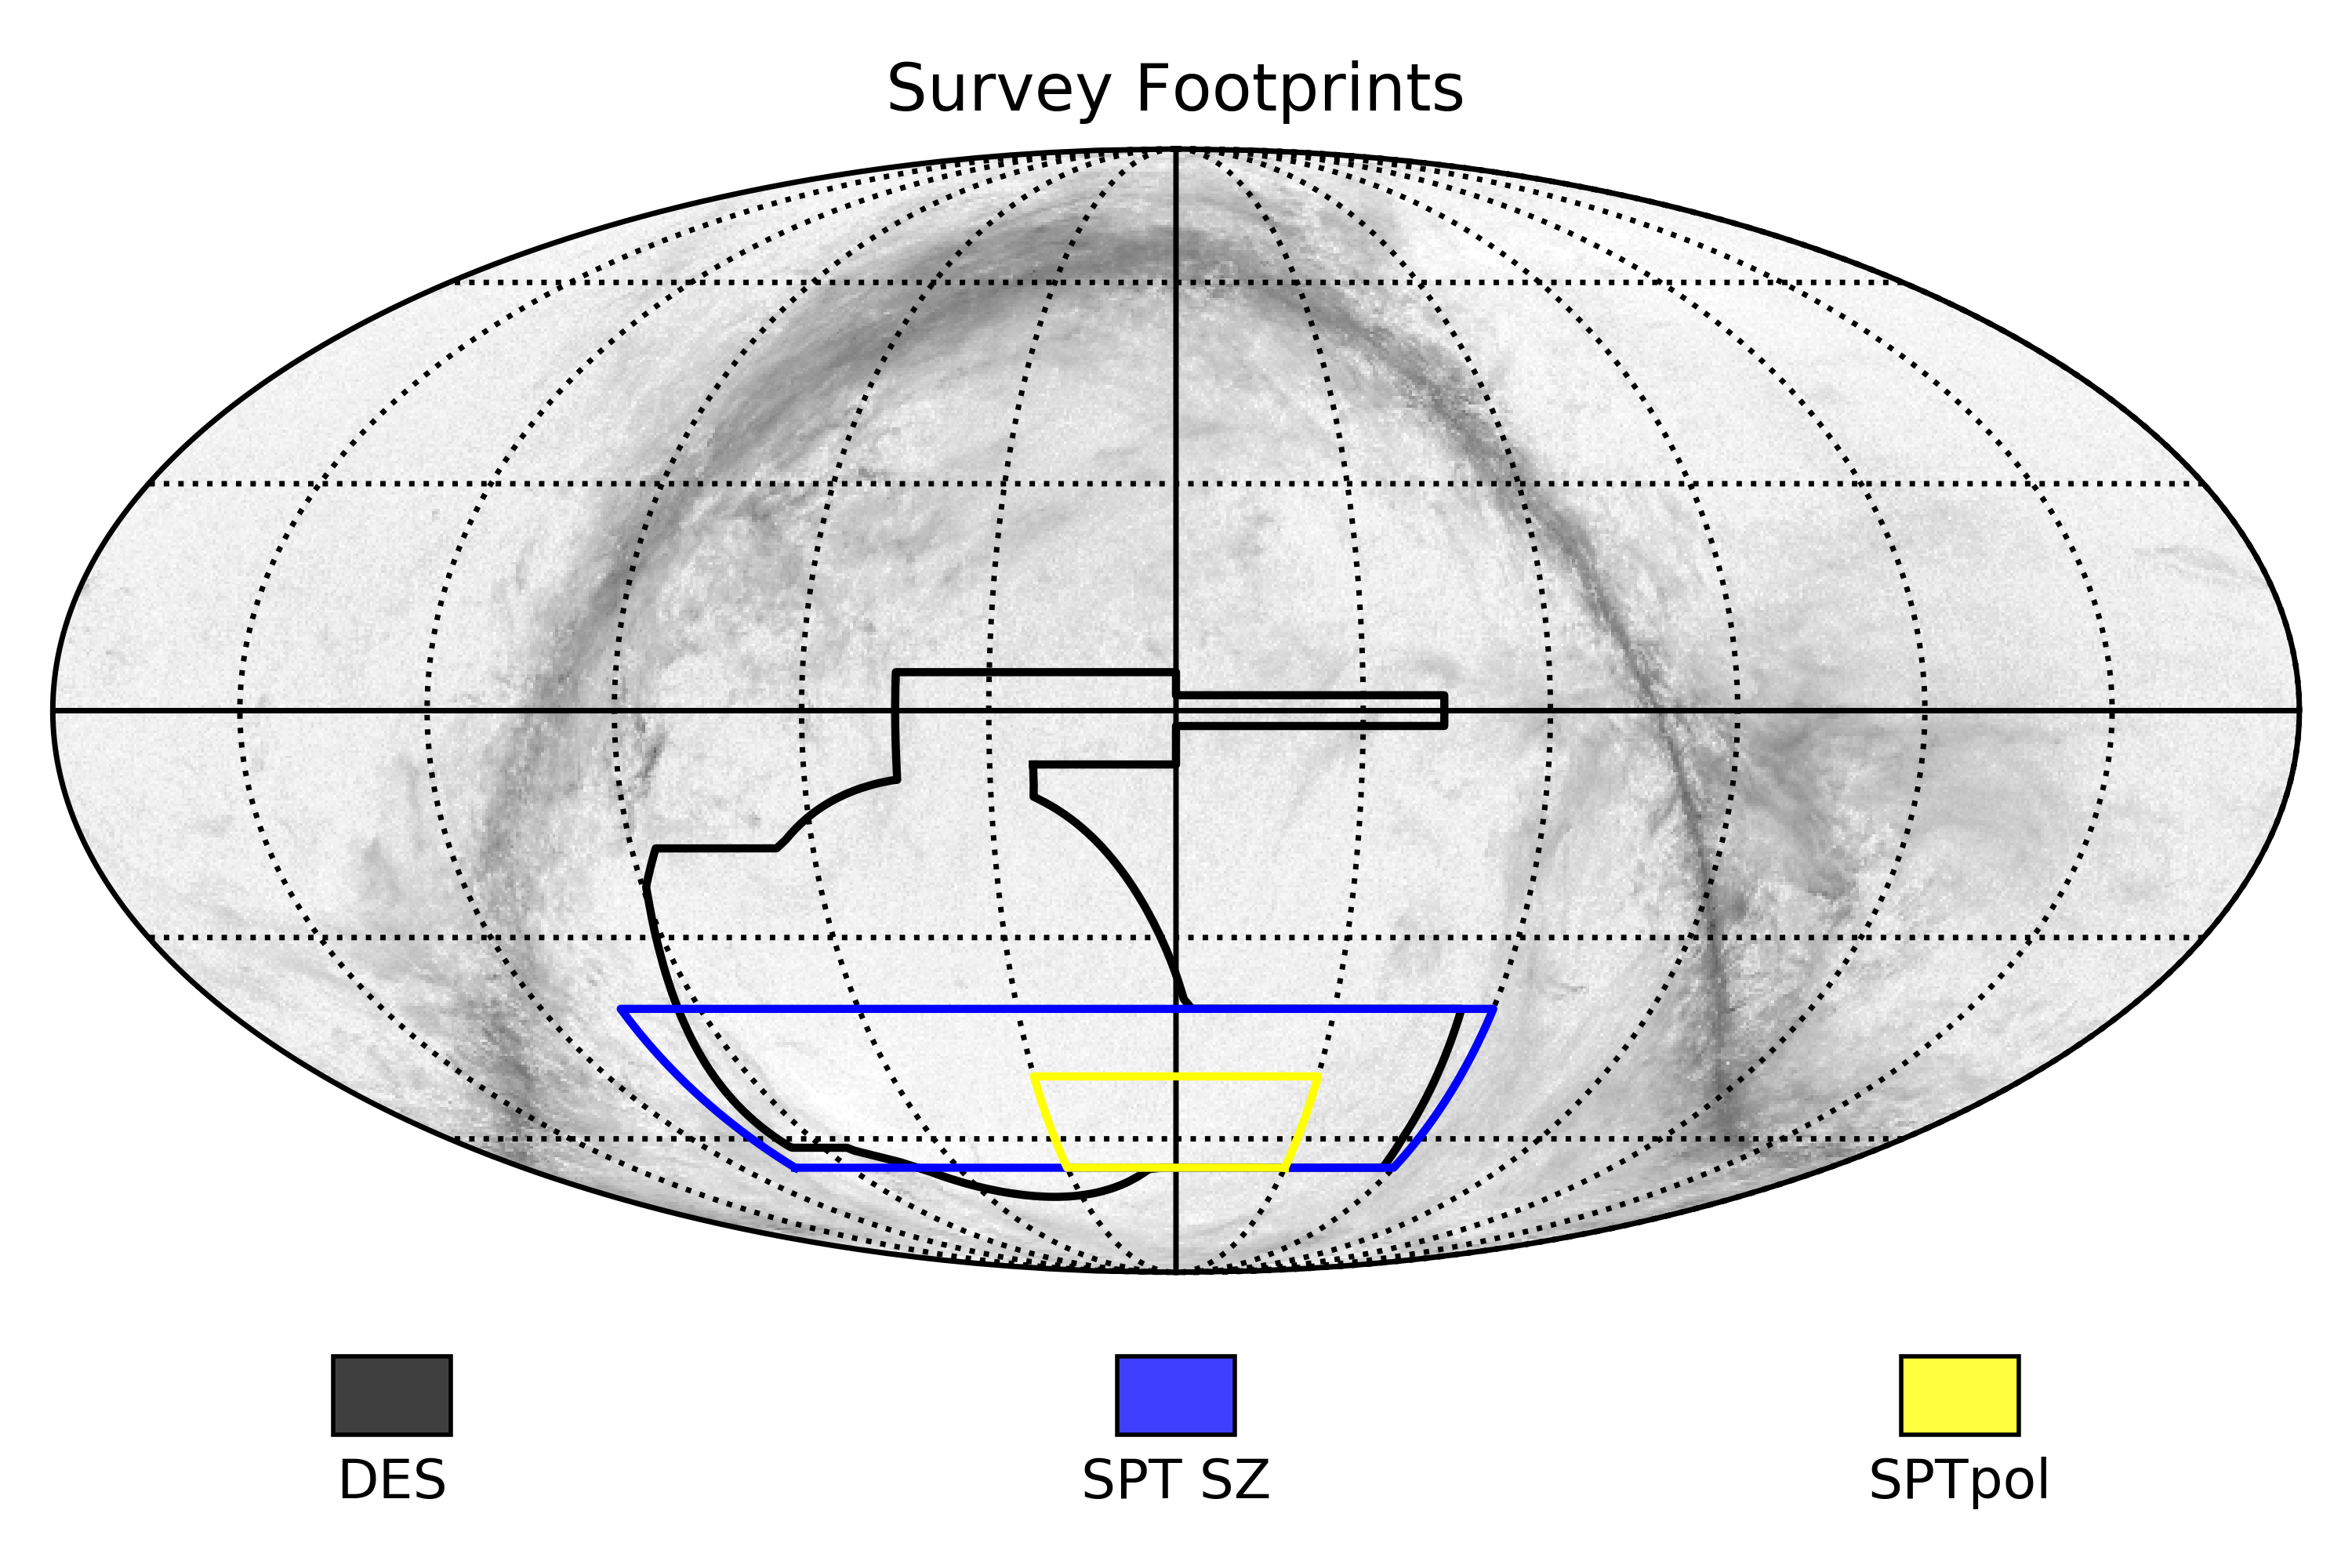
\includegraphics[width=\textwidth , keepaspectratio]{/home/mitchell/Documents/masters/masters/thesis/Ver_2/figures/Survey_Outlines.png}
\caption{Outlines of SPTpol, SPT-SZ, and DES surveys}
\label{fig:surveys}
\end{figure}

Pairs were generated by making use of kD-trees. A generalisation of a binary tree, the kD tree is one where every leaf node is representative of a $k$ dimensional point. Each non-leaf node is one that 'splits' the space into two parts, whereby points to the left of this hyperplane are represented by the left sub-tree, and to the right are represented by the right sub-tree. When we apply this to our galaxy catalogue, we have to locate any two galaxies which satisfy certain conditions regarding line of sight, and transverse separations. All galaxies in the footprint that is being considered are then placed in a kD tree, and any pair which has a radial comoving separation of less that $20 h^{-1} $ Mpc, and transverse comoving separation range of $4 - 20 h^{-1} $ Mpc is considered to have a filament \citep{2016MNRAS.457.2391C,2005MNRAS.359..272C}.

\subsubsection{Data Preparation Algorithm}
\par The algorithm for producing the catalogue of galaxy pairs is as follows:

\begin{enumerate}%[label=(\Roman*)]
\item Convert DES Right Acensions to usable format. \label{alg:pairs:step:1}
\item Remove any galaxies that are not contained in a given footprint \label{alg:pairs:step:2}
\item Store Locations of Galaxies (as Right Acensions and Declinations) in kD-Tree. \label{alg:pairs:step:3}
\item Search kD-Tree for any point within some chosen distance from a given galaxy (e.g. within $\sim 1 \text{deg}^2$).\label{alg:pairs:step:4}
\item Construct a list of pairs which satisfy this approximate distance condition . \label{alg:pairs:step:5}
\item Convert DES Photometric Redshifts into Comoving Distances.\label{alg:pairs:step:6}
\item Calculate the difference in the comoving distance between a given pair. \label{alg:pairs:step:7}
\item Make cuts to catalogue of galaxy pairs based on chosen line-of-sight separation condition.\label{alg:pairs:step:8}
\item Compute the mean redshift of a given pair \label{alg:pairs:step:9}
\item Compute the actual angular separation of a given pair \label{alg:pairs:step:10}
\item Use \ref{alg:pairs:step:9} to determine the equivalent transverse comoving distance at the redshift given by \ref{alg:pairs:step:8}. \label{alg:pairs:step:11}
\item Make cuts to catalogue of galaxy pairs base on chosen transverse separation conditions.\label{alg:pairs:step:12} 
\end{enumerate}

\par Step \ref{alg:pairs:step:1} is necessary, because there are multiple ways to report one of the two coordinates for sky position, Right Acension (RA), and in order for the kD-Tree algorithm to work, they need to fall into a specific format. They can either be expressed on the domain from $[0,360)$, or $(-180,180]$, and the data as obtained reports the RAs of galaxies in the first format, whilst we need the second. If we tried to run the algorithm on the original data, we would inadvertently exclude any pairs in one half of the footprint with step \ref{alg:pairs:step:2}. It would also prevent pairs from being formed in the left half of the image, since the domain for sky locations would now be discontinuous, and so would register two galaxies which may be right next to each other as having a separation of 360 degrees. 

\par Step \ref{alg:pairs:step:2} ensures that we are not including galaxies which are not contained in the relevant footprint. We also have to be careful to avoid edge effects in the $y$-map. When constructing CMB data products, the edges of the map typically have significantly more noise, since there are fewer passes made of the edges in a given observing run. Typically these pixels are de-weighted when compared to pixels in the centre of the map, but if sufficient observing run maps are co-added together, the effects of the noise should be mitigated. The map we are using has been made by combining two independent data sources, the SPT-SZ, and Planck datasets. This should serve to appropriately reduce edge effects, but it is still something to keep in mind.

\par Step \ref{alg:pairs:step:3} and step \ref{alg:pairs:step:4} are important, because the only way that the kD-Tree functions is if there is some `distance' in kD space from which an initial calculation can be defined. The algorithm starts at a given node and searches down the tree until it moves beyond its defined `distance', then it constructs a pair of every node which falls below this condition. These steps do make an assumption that on small enough scales, the sky is flat, which isn't true in a general sense, but is necessary to construct an initial set of pairs.

\par Step \ref{alg:pairs:step:6} follows the process outlined by \cite{1999astro.ph..5116H}, where the comoving distance at a given redshift is given by 
\begin{equation}
D_C = D_H \int_0^z \frac{dz^\prime}{E(z^\prime)}
\label{eq:comov_dist}
\end{equation}
where $E(z^\prime) = \sqrt{\Omega_M (1+z)^3 + \Omega_k (1+z)^2 + \Omega_\Lambda}$ defines the scale factor at a given redshift, and $D_H \equiv \frac{c}{H_0}$ is the Hubble distance. The scale factor depends on $\Omega_M$, $\Omega_\Lambda$, the dimensionless density parameters describing the proportion of matter and dark energy in the universe, and $\Omega_k = 1 - \Omega_M - \Omega_\Lambda$, which describes the curvature of the universe. This calculation takes into account the curvature effects of the various constituents of the universe, as well as the changing scale factor as you look back.

\par This calculation allows us to make the rather significant cuts to the list of potential pairs quite early. The size of the dataset means that performing all operations on all possible pairs would be very computationally expensive, so making the line of sight cuts early is preferred. 

\par Computing the transverse separation takes a little bit more computation effort, because our earlier assumption of sky-flatness cannot be taken as true. The separation between two events at the same redshift, but separated by some angle on the sky $\delta \theta$ is given by $D_M \delta \theta$, where $D_M$ is the comoving transverse distance at the redshift in question. For a flat universe ($\Omega_k = 0$), the comoving transverse distance is equivalent to the comoving line of sight distance (i.e. $D_M = D_C$), but this number is fundamentally dependent on the chosen cosmology. Because of the changing scale factor, objects at different redshifts with the same size will have different angular extents, so this must be taken into account. We do have to make one rather significant approximation here however, because it is very unlikely that both galaxies in a pair might be at the same redshift. As such, we have to approximate their transverse separation at the mean redshift of a given pair. While this approximation is not entirely accurate, it is sub-dominant to the uncertainty on photometric redshifts provided by DES. 


\subsubsection{Data Analysis Algorithm} \label{alg:analysis}
Functionally, this algorithm follows some elementary primary operations:
\begin{enumerate}%[label=(\Roman*)]
\item A pair is located in the CMB \label{alg:stack:step:1}
\item A slice is taken around the pair \label{alg:stack:step:2}
\item The slice is then rotated, so that the pair is aligned along the same axis \label{alg:stack:step:3}
\item The slice is then rescaled, so that each element of the pair is situated at the same point in pixel space \label{alg:stack:step:4}
\item These slices are then mirrored, in both the $x$ and $y$ axes separately and then together, and the average is taken over all four mirror images \label{alg:stack:step:5}
\item These averages are then co-added, and the average is taken over the number of pairs added together \label{alg:stack:step:6}
\end{enumerate}
%\FloatBarrier

%\begin{figure}[h!]
%\centering 
%\includegraphics[scale=0.8]{/home/mitchell/Documents/masters/masters/data/server/run_42/steps/1_firstcut.png}
%\caption{Initial Slice of CMB}
%\label{fig:first_cut}
%\end{figure}

Steps \ref{alg:stack:step:5} and \ref{alg:stack:step:6} are done by applying an affine transformation to the array of values, because we are seeking to preserve the functional position of all points, straight lines, and ratios in the array, as close to the original as possible. This transformation effectively involves applying a transformation matrix to a given image or array, and applying a spline interpolation if there isn't a perfect transformation between the inital and final state.

%\begin{figure}[h!]
%\centering 
%\includegraphics[scale=0.8]{/home/mitchell/Documents/masters/masters/data/server/run_42/steps/1_rotated.png}
%\caption{Rotated Cut-Out}
%\label{fig:rotated}
%\end{figure}


%\begin{figure}[h!]
%\centering 
%\includegraphics[scale=0.8]{/home/mitchell/Documents/masters/masters/data/server/run_42/steps/1_rescaled.png}
%\caption{Rescaled Cut-Out}
%\label{fig:rescaled}
%\end{figure}

 
%\begin{figure}[h!]
%\centering 
%\includegraphics[scale=0.8]{/home/mitchell/Documents/masters/masters/data/server/run_42/steps/1_secondcut.png}
%\caption{Second Cut-Out}
%\label{fig:second_cut}
%\end{figure}

We perform operations \ref{alg:stack:step:4} and \ref{alg:stack:step:5} because we make the assumption that the dark matter halos that host the LRGs we are considering are spherically symmetric. Mirroring the halos about two axes essentially allows us to stack multiple versions of each individual halo. Doing so reduces irregularities introduced by any halos that happen to be non-symmetric, whilst correlating their spherical structure. 

We tested this algorithm by creating dummy simulated datasets, where an artifical signal inserted in noise that is 3 to 4 orders of magnitude higher than it. 

\begin{figure}[h!]
\begin{center}

\includegraphics[width=\textwidth , keepaspectratio]{/home/mitchell/Documents/masters/masters/thesis/Ver_2/figures/simulated_stack.png}
\caption{Stacking Algorithm as applied to Dummy Data. (a) Slice is taken of a given pair, (b) Slice is rotated, aligning both elements of the pair with the $x$ axis, (c) Slice is rescaled. Axes scales have been left in to illustrate the relative scaling between (b) and (c), (d) Second slice is taken of the manipulated data}
\end{center}
\end{figure}

As can be clearly seen, there appears to be no signal in the individual slices of data, but when they are coadded and mirrored, the signals clearly appear as two bright halos. 

Some things to note about this method. First, there are some interesting artefacts along the lines of symmetry. Because both signal and noise are getting mirrored about two axes, any data that lies along one of these axes will get flipped, but will not move in place. This introduces some measure of artificial correlation, because any noise that lies along these axes will look like it is correlated with the un-mirrored data. This is clear in artefacts that lie along the vertical axis. 
%\begin{figure}
%\centering
%\includegraphics[scale=1]{/home/mitchell/Documents/masters/masters/data/server/run_42/steps/1_average.png}
%\caption{Average of Mirrored Arrays}
%\label{fig:average_cut}
%\end{figure}
Secondly, it is sensitive to the separation of the galaxy pair in pixel space. If a galaxy is relatively close together, the rescaling operation will stretch out the pair until they are located at the normalised positions chosen. This also has the effect of stretching out their halo as a whole. This means that pairs that are more separated in pixel space will be rescaled less, and so the halos will be more compact, and pairs that have a lower separation will be rescaled more, and so have a larger angular extent after rescaling. This essentially means that the halo sizes will not be evenly distributed, they will follow the distribution of the pair separations on the sky.  

\par Once we have the pairs co-added, we need to subtract the halo contribution. There are a number of possible ways to do this. We can analytically solve for the halo contribution in the map by using a model of the form 
\begin{equation}
y_h(p) = y_{L,i} + y_{R,j},
\end{equation}
where $p$ represents a given pixel, $L$ and $R$ indicate the left and right halos respectively, and $i$ is the $i$th radial bin from the centre of the left halo, and $j$ is the $j$th radial bin from the centre of the right halo. 



%\begin{figure}[h!]
%\centering 
%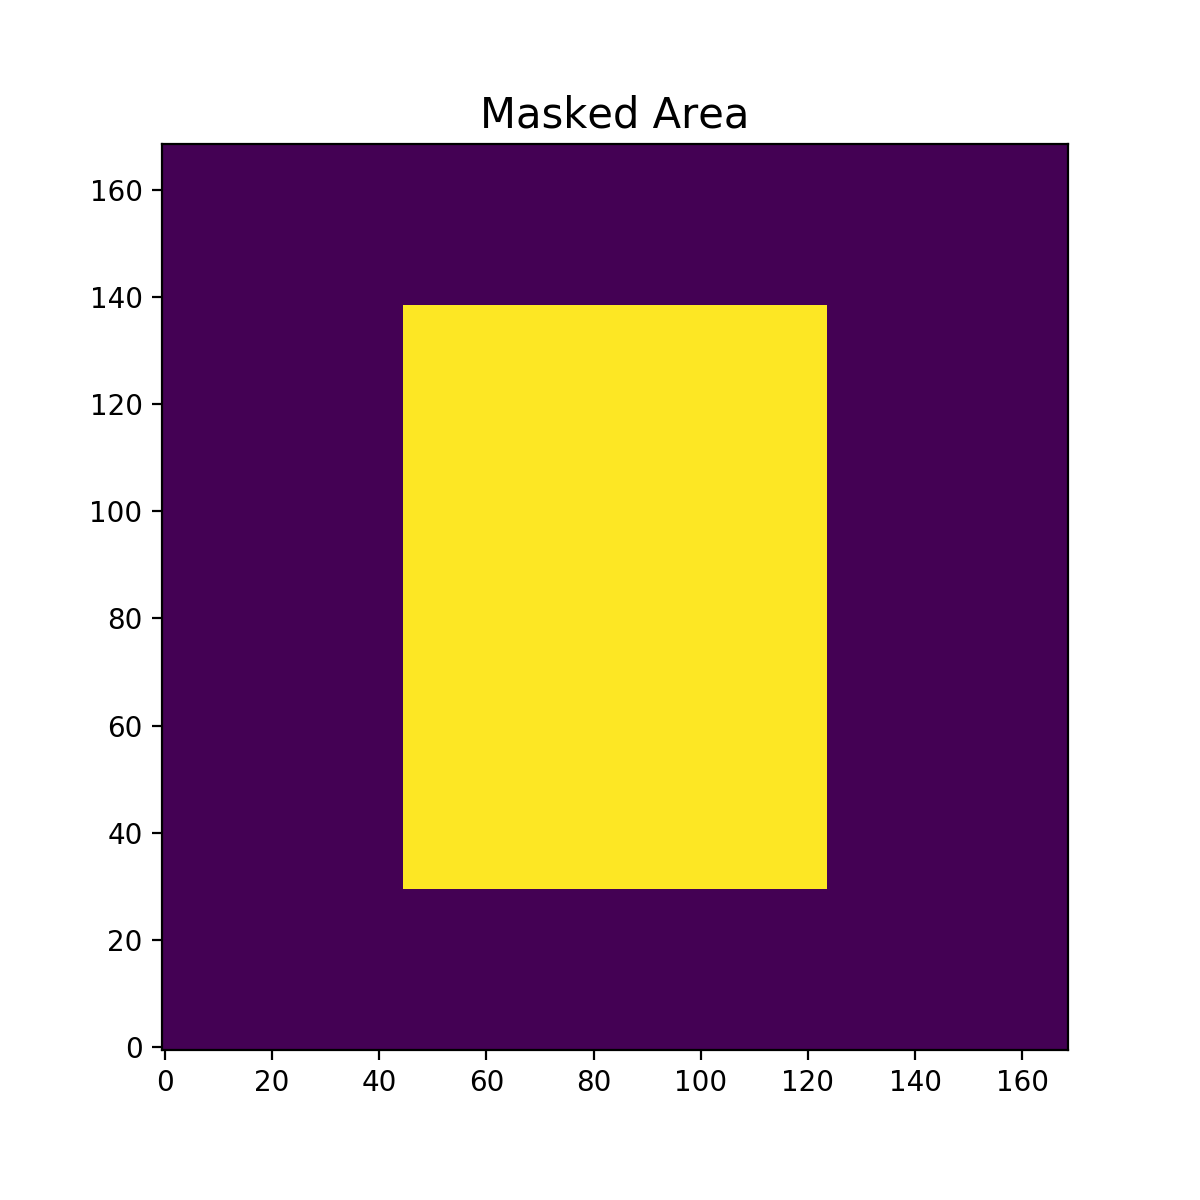
\includegraphics[width=0.6\textwidth , keepaspectratio]{/home/mitchell/Documents/masters/masters/thesis/Ver_2/figures/mask.png}
%\caption{Area of galaxy pair stack masked from profile fit. Masked pixels are in yellow.}
%\label{fig:fit_mask}
%\end{figure}

\par We now have to consider our model choice. Naively, we can model the halos simply by computing the radial profile of one of the halos, and excluding regions which will have a minimal contribution from the secondary halo. We can then assume some background level, and subtract that model away from our signal. 

\par If we want to truly take into account both halo contributions at a given pixel however, we need to calcualte the model in a 2D space. There are two primary models that we can consider here, with a number of possible variations. Given that we have assumed that the halos are mostly spherically symmetric, it follows that they may take the form of Gaussian profiles, so we can consider a model which places two gaussians in the positions of the two halos. 
\par The second model we consider is a fourth order polynomial model, with some form of suppression. This second model takes into account the possibility that the functional form of the halos needs to decay faster than a polynomial ordinarily would, but allows for some flexibility of shape that is not afforded by the gaussian model.

\par We initially consider the models in one dimension, along the effective centre of the galaxy halo pairs. This makes sense if the assumption holds that the galaxy halos are spherical to some leading order. If this assumption doesn't hold for any reason, either physical, or one introduced by our algorithm, we should consider performing our fit over the entirety of the two dimensional image produced by the stack. Whether this will be effective is ultimately dependant on the level of symmetry in the stack, and how well the two dimensional fit performs. In order to avoid introducing bias from the potential filament, we exclude the central region of the stack, as shown in Figure \ref{fig:fit_mask}

\par Once these models have been fitted, and subtracted from our detected signal appropriately, we hope to be left with a filament detection. This will have an average comptonisation, and so will act as a means to measure the amount of matter contained within the WHIM filaments connecting galaxy pairs. 



\section{Null Tests}

In order to test the validity of the detection, and make an estimate of its uncertainty, we perform several different types of Monte-Carlo based tests. 

\subsection{Un-Physical Pairs}
The first test involves stacking the $y$ map against 'pseudo-pairs' of galaxies. These pairs satisfy the transverse separation condition, but do not satisfy the radial separation condition, having instead radial separations between $\SI{100}{\per\h}$ and $\SI{200}{\per\h}$ Mpc. Pairs with these conditions are not expected to have any filament connecting them, and the radial separation conditions have been calculated to take into account the errors associated with the photometric redshifts found in the Dark Energy Survey catalogue. 
\par In order to produce this pair set, we first calculate the total number of pairs that sit within approximately $\SI{1}{\degree}$ on the sky, and calculate their line of sight separations. We then determine the transverse separation of the pair, and apply the same cuts as for the physical pairs. 
\par Once these pairs are stacked, they should show a map that is similar to the physical pairs, but with visibly less signal between the two halos, where we expect to see the signal. 
\par If we perform the same halo fit as for the physical pairs, we should be able to subtract the halo contributions for this dataset and see no visible filament signal. 
\subsection{Random Stack}
The second test involves creating a random stack of CMB slices, to estimate the RMS of the background. At first glance, this would suggest just randomly sampling points inside the footprint of both surveys. However, because there is contamination in the CMB, in the form of various foregrounds, we have to ensure that the noise introduced by this is going to be the same as for the physical pairs. Given that the noise in the CMB is approximately constant at a given galactic latitidue, we can therefore randomly select a point that is at the same galactic latitude as a given pair, but with some random longitude. We would expect, given that the fluctuations in the CMB are approximately gaussian, that this stack would have no discernable structure.